\section{Motivation}

Die Elektrolyse wurde erstmals im Jahr 1800 entdeckt durch Alessandro Volta. Dieser stellte die erste brauchbare Batterie her.
In den darauffolgenden Jahren konnten mithilfe der Elektrolyse erstmals elementare unedle Metalle hergestellt werden. \\
Im Alltag präsent ist die Elektrolyse in Batterien, aber auch in Aluminium.
Um Aluminium elementar extrahieren zu können wird die Elektrolyse verwendet. Aluminium ist in der heutigen Zeit ein weitverbreitetder
Werkstoff, da es sehr leicht, aber auch stabil ist.

\section{Messverfahren}
Der Verscuh besteht aus drei Aufbauten:\\
\begin{itemize}
    \item Einer Elektrolysezelle aus zwei Kupferplatten und einem Kupfer-Sulfat Elektrolyt. Dabei wird Strom an die Kupferplatten gelegt. Durch den Strom
    scheidet sich an einer Platte elementares Kupfer ab, wärend bei der anderen Kupfer als Ion in Lösung geht. Aus der Massendifferenz der Platten vor und nach der Elektrolyse kann die Faraday-Kosntante bestimmt werden.
    \item Einer Elektrolysezelle mit zwei Platin Elektroden und Wasser. Durch den Strom entstehen elementarer Sauer- und Wasserstoff. Durch die Volumendifferenz zum Moment vor der Elektrolyse
    lässt sich hier ebenfalls die Faraday-Konstante bestimmen.
    \item Einer Brennstoffzelle, welche mithilfe von elementarem Wasserstoff und Luftsauerstoff, durch Rückreaktion der obigen Elektrolyse, Strom generieren kann.
\end{itemize}



\section{Grundlagen aus der Physik}
Allgemein gilt bei der Elektrolyse folgender Zusammenhang:

\begin{equation}
    n = \frac{Q}{zF}
    \label{eq:eF}
\end{equation}


\subsection{Elektrolyse Kupfersulfat}
Bei der Elektrolyse der Kupferplatten wird die Masse $m$ des sich abgesetzten und gelösten Kupfer gemessen.
Daraus kann mit der bekannten molaren Masse von $M_{Mol} = 63,546 \tfrac{\text{g}}{\text{mol}}$ die Stoffmenge $n$ bestimmt werden:

\begin{equation}
    m = nM_{Mol}
    \label{eq:m}
\end{equation}

Da der Strom $I$ im Verläufe der Elektrolyse nahezu konstant bleibt gibt sich hier der Zusammenhang für die übertragene Ladung $Q$
über die Elektrolysezeit $t$:
\begin{equation}
    Q = It
\end{equation}

Setzt man diese bein Formeln in die Allgemeine Formel \ref{eq:eF} ein, erhält man einen Ausdruck für die Faraday-Konstante $F$:

\begin{align}
    F &= \frac{Q}{zm}M_{Mol} \\
    \Leftrightarrow F &=  \frac{It}{zm}M_{Mol}
    \label{eq:FCu}
\end{align}


\subsection{Elektrolyse Wasser}

Bei der Elektrolyse von Wasser zu $H_2$ und $O_2$ wird nicht die Massendifferenz, sonder die Volumendifferenz $V$ bestimmt.
Hie muss zur Bestimmung der Faraday-Konstante erneut die Stoffmenge bestimmt werden.
Dafür gilt in dem Fall der Volumenmessung:
\begin{equation}
    n = \frac{V}{V_{Mol}}
    \label{eq:n}
\end{equation}

Dabei ist $V_{Mol}$ das Molvolumen, welches das Volumen von einem mol eines Idealen Gases angibt.
Dieses kann über das ideale Gasgesetz hergeleitet werden mit $p$ als Druck,$T$ als Temperatur,
$p_0 = 1013,25\  \text{mbar}$ und $T_0 = 273,15\ \text{K}$ als Normalbedingungen und $V_{Mol}^0 = \SI{22,414}{\litre \per \mole}$ als Molvolumen unter Normalbedingungen:

\begin{equation}
    V_{Mol} = \frac{p_0}{p}\frac{T}{T_0}V_{Mol}^0
    \label{eq:VMol}
\end{equation}

Da sich in dem Wasser noch verdünnte Schwefelsäure $H_2SO_4$ befindet, darf nur der
Partialdruck des jeweiligen Gases berücksichtigt werden. Dabei wird der Sättigungsdruck des Elektrolyts
mit 90 \% von dem Sättigungsdruck von reinem Wasser geschätzt.
Damit folt dann für den Druck $p$, mit dem Luftdruck $p_L$ und den Sättigungsdrücken
$p_D^{H_2SO_4}$ für das Elektrolyt und $p_D^{H_2O}$ für den Sättigungsdruck von reinem Wasser:

\begin{align}
    p &= p_L - p_D^{H_2SO_4}\\
    \Leftrightarrow p &= p_L - 0,9 \cdot p_D^{H_2O}
    \label{eq:p}
\end{align}

Eigentlich müsste noch der hydrostatische Druck berücksichtigt werden, da aber der Behälter beim messen auf höhe des Wasserspiegels der Röhren gebracht wurde, fällt deiser in der Berechnung weg.
\newpage
\section{Aufbau}
\begin{figure}[h!]
    \centering
    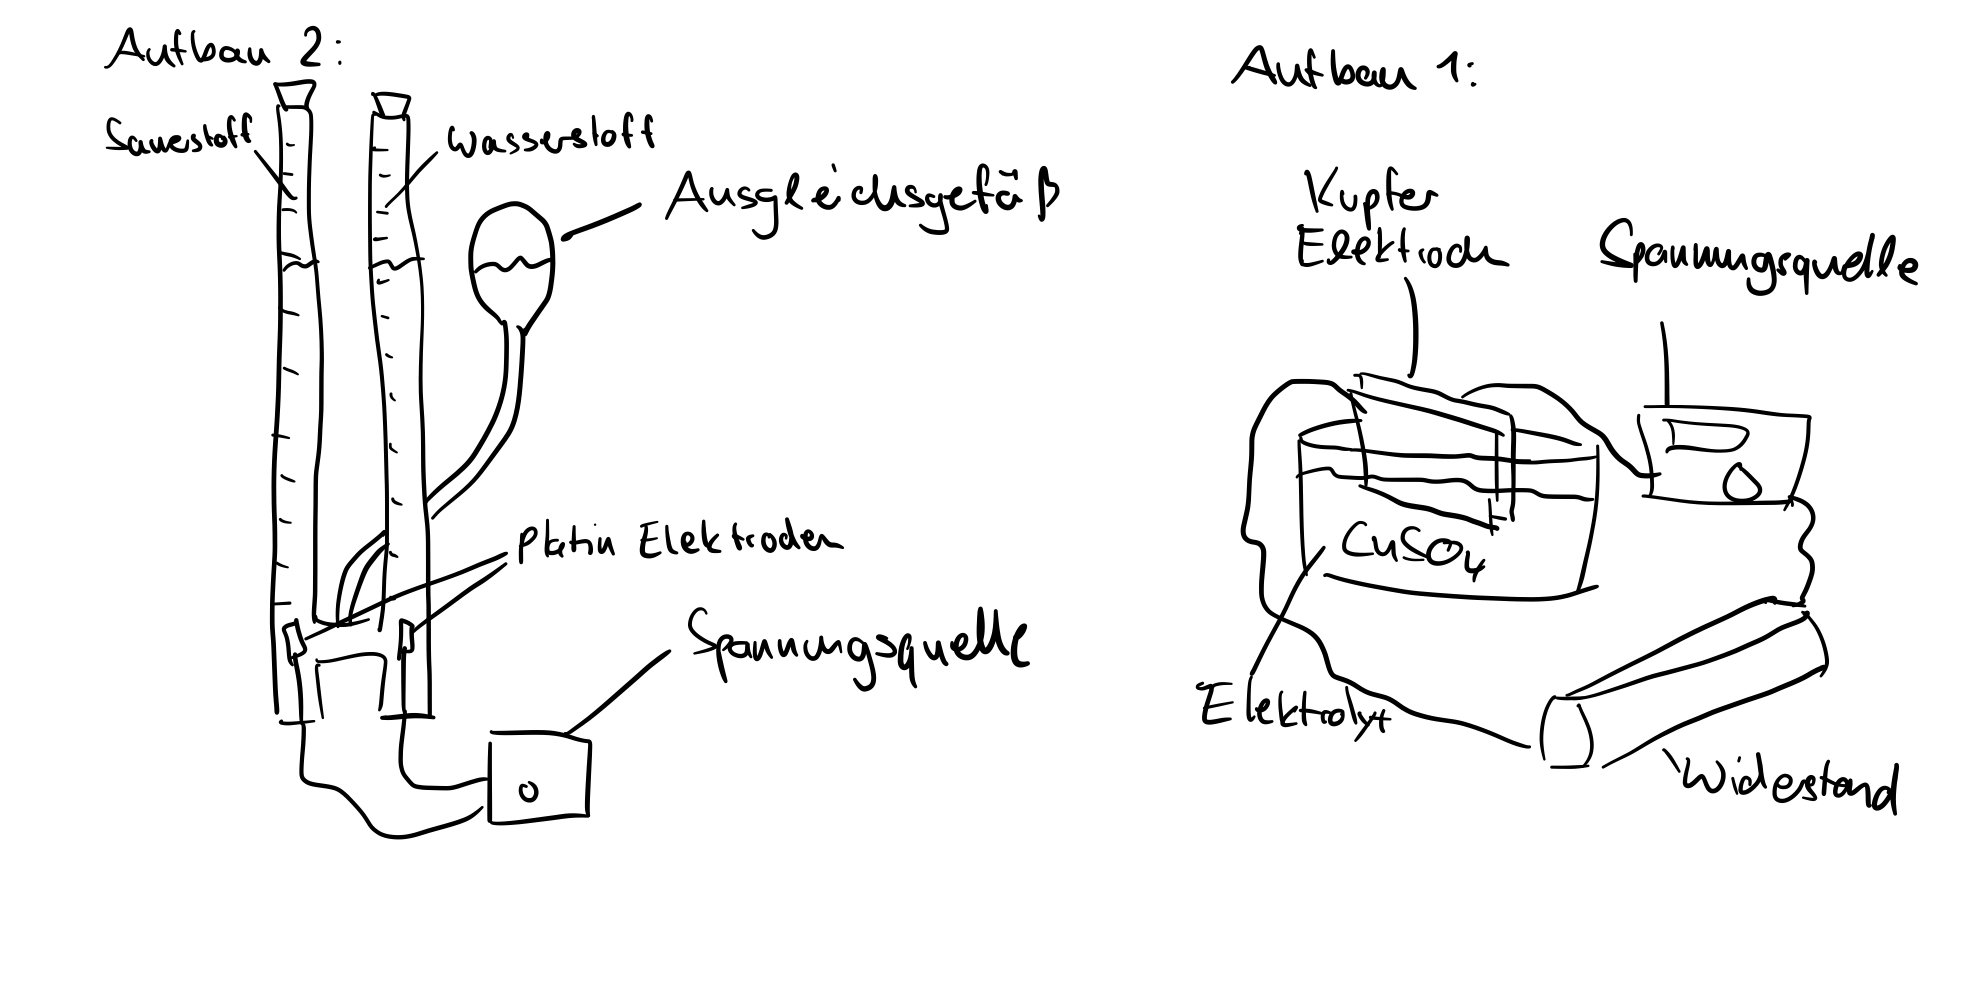
\includegraphics[width = .8\textwidth]{Aufbau.jpeg}
    \caption{Aufbau}
\end{figure}
\clearpage
\newpage
